\section{Peta Karnaugh 3 Variabel}

Peta Karnaugh 3 variabel terdiri dari $2^3 = 8$ sel yang disusun dalam grid berukuran $2 \times 4$. Satu variabel ditempatkan pada sumbu baris, sedangkan dua variabel lainnya ditempatkan pada sumbu kolom menggunakan urutan Kode Gray. Pada konfigurasi ini, properti \textit{wrap-around} mulai berperan: sel pada kolom paling kanan secara logis bersebelahan dengan sel pada kolom paling kiri, karena label Gray-nya hanya berbeda satu bit \cite{rosen2019}.

\subsection{Struktur dan Pemetaan Minterm}

Gambar~\ref{fig:kmap-3var} menampilkan struktur K-Map 3 variabel dengan variabel $X$ pada baris dan variabel $Y, Z$ pada kolom. Perhatikan urutan kolom mengikuti Kode Gray: $00, 01, 11, 10$ (bukan urutan biner biasa $00, 01, 10, 11$).

\begin{figure}[H]
\centering
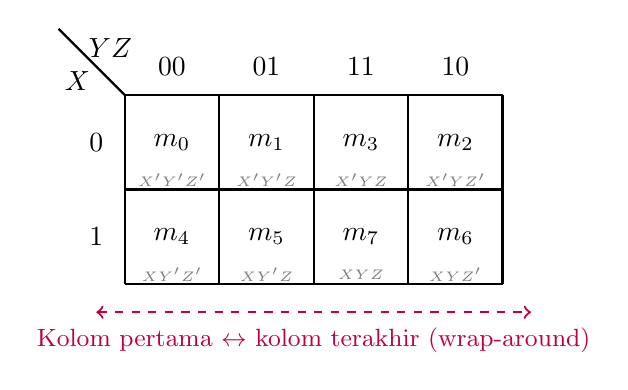
\begin{tikzpicture}[scale=1.2]
    % Grid 4x2
    \draw[thick] (0,0) grid (4,2);
    % Diagonal divider
    \draw[thick] (0,2) -- (-0.7,2.7);
    \node at (-0.5, 2.15) {$X$};
    \node at (-0.15, 2.5) {$YZ$};
    % Column Labels (Gray Code)
    \node at (0.5, 2.3) {$00$}; \node at (1.5, 2.3) {$01$}; \node at (2.5, 2.3) {$11$}; \node at (3.5, 2.3) {$10$};
    % Row Labels
    \node at (-0.3, 1.5) {$0$}; \node at (-0.3, 0.5) {$1$};
    % Cells
    \node at (0.5, 1.5) {$m_0$}; \node at (1.5, 1.5) {$m_1$}; \node at (2.5, 1.5) {$m_3$}; \node at (3.5, 1.5) {$m_2$};
    \node at (0.5, 0.5) {$m_4$}; \node at (1.5, 0.5) {$m_5$}; \node at (2.5, 0.5) {$m_7$}; \node at (3.5, 0.5) {$m_6$};
    % Small labels
    \node[font=\tiny, gray] at (0.5, 1.1) {$X'Y'Z'$}; \node[font=\tiny, gray] at (1.5, 1.1) {$X'Y'Z$};
    \node[font=\tiny, gray] at (2.5, 1.1) {$X'YZ$}; \node[font=\tiny, gray] at (3.5, 1.1) {$X'YZ'$};
    \node[font=\tiny, gray] at (0.5, 0.1) {$XY'Z'$}; \node[font=\tiny, gray] at (1.5, 0.1) {$XY'Z$};
    \node[font=\tiny, gray] at (2.5, 0.1) {$XYZ$}; \node[font=\tiny, gray] at (3.5, 0.1) {$XYZ'$};
    % Wrap-around indicator
    \draw[<->, thick, purple, dashed] (-0.3, -0.3) -- (4.3, -0.3);
    \node[purple, font=\small] at (2, -0.6) {Kolom pertama $\leftrightarrow$ kolom terakhir (wrap-around)};
\end{tikzpicture}
\caption{Struktur Peta Karnaugh 3 Variabel dengan Indikasi Wrap-Around}
\label{fig:kmap-3var}
\end{figure}

Perhatikan bahwa kolom $00$ dan kolom $10$ hanya berbeda pada satu bit (bit $Y$), sehingga secara logis bersebelahan meskipun terletak pada tepi yang berlawanan pada peta. Kelompok yang mencakup sel-sel pada kedua tepi ini tetap valid selama memenuhi aturan pengelompokan.

\subsection{Contoh Penyederhanaan Langkah demi Langkah}

\begin{contoh}
\textbf{Penyederhanaan $F(X,Y,Z) = \sum m(1, 3, 5, 7)$}

\textbf{Langkah 1:} Tempatkan nilai 1 pada K-Map:

\begin{center}
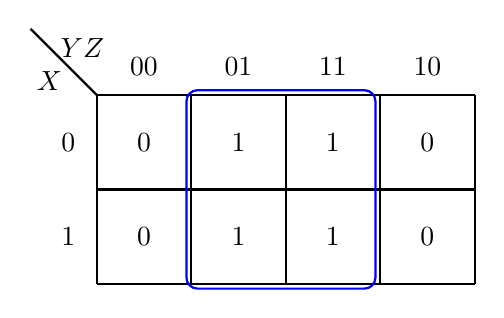
\begin{tikzpicture}[scale=1.2]
    \draw[thick] (0,0) grid (4,2);
    \draw[thick] (0,2) -- (-0.7,2.7);
    \node at (-0.5, 2.15) {$X$};
    \node at (-0.15, 2.5) {$YZ$};
    \node at (0.5, 2.3) {$00$}; \node at (1.5, 2.3) {$01$}; \node at (2.5, 2.3) {$11$}; \node at (3.5, 2.3) {$10$};
    \node at (-0.3, 1.5) {$0$}; \node at (-0.3, 0.5) {$1$};
    % Values
    \node at (0.5, 1.5) {0}; \node at (1.5, 1.5) {1}; \node at (2.5, 1.5) {1}; \node at (3.5, 1.5) {0};
    \node at (0.5, 0.5) {0}; \node at (1.5, 0.5) {1}; \node at (2.5, 0.5) {1}; \node at (3.5, 0.5) {0};
    % Group: all cells with Z=1
    \draw[thick, blue, rounded corners] (0.95, -0.05) rectangle (2.95, 2.05);
\end{tikzpicture}
\end{center}

\textbf{Langkah 2:} Identifikasi kelompok. Keempat sel bernilai 1 ($m_1, m_3, m_5, m_7$) membentuk satu kelompok berukuran 4 pada dua kolom tengah.

\textbf{Langkah 3:} Eliminasi variabel. Di dalam kelompok ini:
\begin{itemize}
    \item $X$ berubah ($0 \rightarrow 1$): dieliminasi
    \item $Y$ berubah ($0 \rightarrow 1$): dieliminasi
    \item $Z = 1$ konstan: dipertahankan
\end{itemize}

\textbf{Hasil}: $F = Z$

Verifikasi: $m_1 = X'Y'Z$, $m_3 = X'YZ$, $m_5 = XY'Z$, $m_7 = XYZ$. Semua minterm memiliki $Z = 1$, sehingga faktor persekutuannya adalah $Z$.
\end{contoh}

\begin{contoh}
\textbf{Penyederhanaan $F(X,Y,Z) = \sum m(0, 2, 4, 5)$ dengan Wrap-Around}

\textbf{Langkah 1:} Tempatkan nilai 1 pada K-Map:

\begin{center}
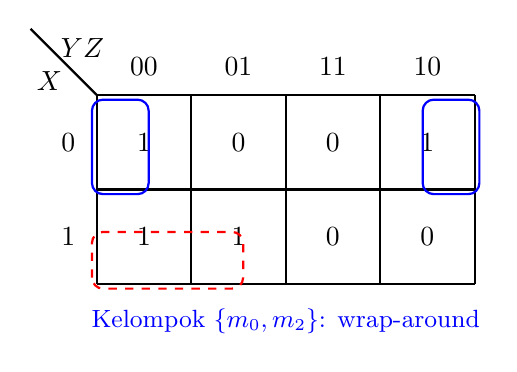
\begin{tikzpicture}[scale=1.2]
    \draw[thick] (0,0) grid (4,2);
    \draw[thick] (0,2) -- (-0.7,2.7);
    \node at (-0.5, 2.15) {$X$};
    \node at (-0.15, 2.5) {$YZ$};
    \node at (0.5, 2.3) {$00$}; \node at (1.5, 2.3) {$01$}; \node at (2.5, 2.3) {$11$}; \node at (3.5, 2.3) {$10$};
    \node at (-0.3, 1.5) {$0$}; \node at (-0.3, 0.5) {$1$};
    % Values
    \node at (0.5, 1.5) {1}; \node at (1.5, 1.5) {0}; \node at (2.5, 1.5) {0}; \node at (3.5, 1.5) {1};
    \node at (0.5, 0.5) {1}; \node at (1.5, 0.5) {1}; \node at (2.5, 0.5) {0}; \node at (3.5, 0.5) {0};
    % Group 1: wrap-around (m0, m2, m4) -> actually m0 and m2 wrap around
    \draw[thick, blue, rounded corners] (-0.05, 0.95) rectangle (0.55, 1.95);
    \draw[thick, blue, rounded corners] (3.45, 0.95) rectangle (4.05, 1.95);
    \node[blue, font=\small] at (2, -0.4) {Kelompok $\{m_0, m_2\}$: wrap-around};
    % Group 2: m4, m5
    \draw[thick, red, rounded corners, dashed] (-0.05, -0.05) rectangle (1.55, 0.55);
\end{tikzpicture}
\end{center}

\textbf{Langkah 2:} Identifikasi kelompok:
\begin{itemize}
    \item \textcolor{blue}{Kelompok 1}: $\{m_0, m_2\}$ --- wrap-around, $X = 0$ dan $Z = 0$ konstan, $Y$ berubah $\Rightarrow$ suku: $X'Z'$
    \item \textcolor{red}{Kelompok 2}: $\{m_4, m_5\}$ --- $X = 1$ dan $Y = 0$ konstan, $Z$ berubah $\Rightarrow$ suku: $XY'$
\end{itemize}

\textbf{Hasil}: $F = X'Z' + XY'$
\end{contoh}

\subsection{Pola Kelompok Umum pada K-Map 3 Variabel}

Beberapa pola pengelompokan yang sering muncul pada K-Map 3 variabel patut diperhatikan. Kelompok berukuran 2 mengeliminasi 1 variabel, kelompok berukuran 4 mengeliminasi 2 variabel, dan kelompok berukuran 8 (seluruh peta) mengeliminasi semua 3 variabel, menghasilkan $F = 1$ (tautologi). Pola \textit{wrap-around} sering terabaikan, sehingga identifikasi kedekatan logis antar sel pada tepi peta memerlukan pengecekan teliti \cite{wiki_karnaugh}.
